\documentclass[tikz, border=14pt]{standalone}
\usepackage{tikz}
\usepackage{amsmath,amssymb}
\usetikzlibrary{arrows.meta, positioning, fit, backgrounds, calc}

\definecolor{imgblue}{HTML}{DBEAFE}
\definecolor{imgborder}{HTML}{3B82F6}
\definecolor{txtgreen}{HTML}{DCFCE7}
\definecolor{txtborder}{HTML}{22C55E}
\definecolor{predorange}{HTML}{FEF3C7}
\definecolor{predborder}{HTML}{F59E0B}
\definecolor{lossred}{HTML}{FFE4E6}
\definecolor{lossborder}{HTML}{F43F5E}
\definecolor{sigpurple}{HTML}{F3E8FF}
\definecolor{sigborder}{HTML}{A855F7}
\definecolor{embgray}{HTML}{F1F5F9}
\definecolor{emborder}{HTML}{94A3B8}

\tikzset{
  block/.style={
    rectangle, rounded corners=4pt,
    minimum width=2.0cm, minimum height=0.85cm,
    align=center, font=\small\bfseries, line width=0.8pt,
  },
  imgenc/.style={block, fill=imgblue,    draw=imgborder},
  txtenc/.style={block, fill=txtgreen,   draw=txtborder},
  predbl/.style={block, fill=predorange, draw=predborder},
  lossbl/.style={block, fill=lossred,    draw=lossborder, font=\small},
  sigbl/.style={ block, fill=sigpurple,  draw=sigborder,  font=\small},
  emb/.style={
    circle, draw=emborder, fill=embgray,
    minimum size=0.75cm, font=\small, line width=0.7pt,
  },
  arr/.style={-{Stealth[length=5pt]}, line width=0.9pt, gray!70!black},
  darr/.style={-{Stealth[length=4pt]}, line width=0.7pt, dashed, gray!55},
  lbl/.style={font=\footnotesize\itshape, text=gray!60!black},
}

\begin{document}
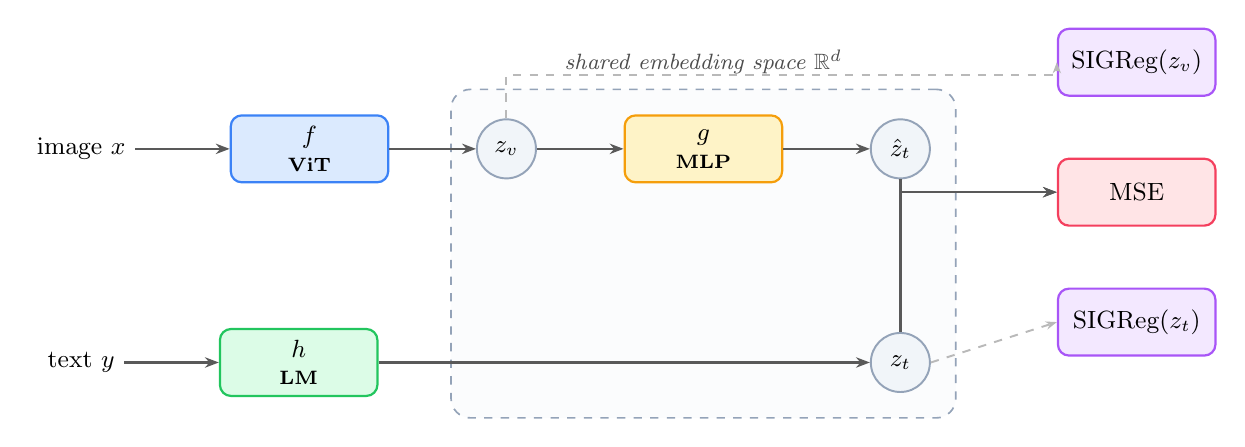
\begin{tikzpicture}[node distance=0.9cm and 1.4cm]

% ── top row: image path ────────────────────────────────────────────────
\node[font=\small] (img) {image $x$};
\node[imgenc, right=1.2cm of img] (vit) {$f$\\[-1pt]{\scriptsize ViT}};
\node[emb,    right=1.1cm of vit] (zv)  {$z_v$};
\node[predbl, right=1.1cm of zv]  (pred){$g$\\[-1pt]{\scriptsize MLP}};
\node[emb,    right=1.1cm of pred](zhat){$\hat{z}_t$};

% ── bottom row: text path, z_t aligned under zhat ─────────────────────
\node[font=\small, below=2.2cm of img] (txt) {text $y$};
\node[txtenc, right=1.2cm of txt] (lm)  {$h$\\[-1pt]{\scriptsize LM}};
% z_t sits directly below zhat so MSE is a clean vertical comparison
\node[emb] at (zhat |- lm) (zt) {$z_t$};

% ── loss column ────────────────────────────────────────────────────────
\node[sigbl,  right=1.6cm of zhat, yshift= 1.1cm] (sigv) {SIGReg$(z_v)$};
\node[lossbl, right=1.6cm of zhat, yshift=-0.55cm] (mse)  {MSE};
\node[sigbl,  right=1.6cm of zhat, yshift=-2.2cm] (sigt) {SIGReg$(z_t)$};

% ── arrows: inputs → encoders ─────────────────────────────────────────
\draw[arr] (img) -- (vit);
\draw[arr] (txt) -- (lm);

% ── arrows: encoders → embeddings ────────────────────────────────────
\draw[arr] (vit) -- (zv);
% lm goes right to zt (may be longer than top path — use a bent arrow)
\draw[arr] (lm.east) -- (zt.west);

% ── image path through predictor ─────────────────────────────────────
\draw[arr] (zv)   -- (pred);
\draw[arr] (pred) -- (zhat);

% ── MSE: zhat and zt arrive from the left, cleanly ───────────────────
% Both exit their nodes to the right then meet mse from the west
\coordinate (mseW) at (mse.west);
\draw[arr] (zhat.south) |- (mse.west);
\draw[arr] (zt.north)   |- (mse.west);

% ── SIGReg: dashed arrows exit RIGHT from the embedding box ──────────
% For zv: go right past zhat, then up to sigv
\coordinate (exitR) at ($(zhat.east) + (0.4,0)$);
\draw[darr] (zv.north) -- ++(0, 0.55cm) -| (sigv.west);
\draw[darr] (zt.east) -- (sigt.west);

% ── shared embedding space background ────────────────────────────────
\begin{pgfonlayer}{background}
  \node[
    draw=emborder, dashed, rounded corners=7pt,
    fill=embgray!30, line width=0.6pt,
    inner sep=9pt,
    fit=(zv)(pred)(zhat)(zt),
  ] (embbox) {};
\end{pgfonlayer}
\node[lbl, above=0.06cm of embbox]
      {shared embedding space $\mathbb{R}^d$};

\end{tikzpicture}
\end{document}
